\documentclass[11pt,a4paper]{article}
\usepackage[utf8]{inputenc}
\usepackage[T1]{fontenc}
\usepackage{lmodern}
\usepackage{geometry}
\usepackage{hyperref}
\usepackage{amsmath}
\usepackage{amsfonts}
\usepackage{amssymb}
\usepackage{graphicx}
\usepackage{booktabs}
\usepackage{longtable}
\usepackage{xcolor}
\usepackage{listings}
\usepackage{tikz}
\usepackage{pgfplots}
\usepackage{algorithm}
\usepackage{algpseudocode}
\usepackage{fancyhdr}
\usepackage{enumerate}
\usepackage{natbib}

\geometry{margin=1in}
\pgfplotsset{compat=1.18}

\hypersetup{
    colorlinks=true,
    linkcolor=blue,
    filecolor=magenta,      
    urlcolor=cyan,
    pdftitle={Global Data Access System PRD},
    pdfauthor={rmatch Project},
    pdfsubject={Product Requirements Document},
    pdfkeywords={data access, pattern matching, distributed systems, performance}
}

\pagestyle{fancy}
\fancyhf{}
\rhead{Global Data Access System PRD}
\lhead{rmatch Project}
\cfoot{\thepage}

\title{\textbf{Product Requirements Document:\\Global Data Access System}}
\author{rmatch Project Team}
\date{\today}

\begin{document}

\maketitle

\begin{abstract}
This document defines the requirements for a high-performance global data access system capable of efficiently searching, matching, and retrieving information from distributed data sources worldwide. The system leverages rmatch's advanced regular expression matching capabilities to provide scalable, low-latency access to vast amounts of structured and unstructured data while maintaining strict security, privacy, and performance constraints.
\end{abstract}

\newpage
\tableofcontents
\newpage

\section{Executive Summary}

The Global Data Access System (GDAS) represents a revolutionary approach to accessing and processing information from distributed data sources across the globe. Built upon rmatch's high-performance pattern matching engine, GDAS aims to provide unified, efficient, and secure access to diverse data repositories while maintaining sub-second query response times and minimal resource allocation overhead.

\subsection{Vision Statement}
To create the world's most efficient and comprehensive data access platform that democratizes information retrieval while respecting privacy boundaries and maintaining exceptional performance characteristics.

\subsection{Key Success Metrics}
\begin{itemize}
\item Query response time: $< 100ms$ for 95\% of requests
\item Throughput: $> 1M$ concurrent pattern matches per second
\item Data coverage: Access to $> 90\%$ of publicly available structured data
\item Memory efficiency: $< 4GB$ heap usage per query node
\item Availability: 99.99\% uptime across all global regions
\end{itemize}

\section{Problem Statement}

\subsection{Current State Analysis}
The current landscape of data access systems suffers from several critical limitations:

\begin{enumerate}
\item \textbf{Fragmentation}: Data exists in silos across different platforms, APIs, and formats
\item \textbf{Performance Bottlenecks}: Existing solutions rely on backtracking regex engines causing unpredictable latency
\item \textbf{Scalability Constraints}: Current systems cannot efficiently handle the volume and variety of global data
\item \textbf{Security Gaps}: Inadequate privacy controls and data sovereignty compliance
\item \textbf{Integration Complexity}: No unified interface for accessing diverse data sources
\end{enumerate}

\subsection{Market Opportunity}
The global data integration market is projected to reach \$19.3 billion by 2026, with pattern matching and search representing a significant portion of this demand. Organizations require real-time access to distributed information for decision-making, compliance, and innovation.

\section{Requirements}

\subsection{Functional Requirements}

\subsubsection{FR1: Universal Data Source Integration}
\textbf{Description}: The system must integrate with diverse data sources including databases, APIs, file systems, streaming platforms, and web services.

\textbf{Acceptance Criteria}:
\begin{itemize}
\item Support for $>$ 50 different data source types
\item Real-time connection health monitoring
\item Automatic failover and load balancing
\item Schema discovery and adaptation capabilities
\end{itemize}

\subsubsection{FR2: High-Performance Pattern Matching}
\textbf{Description}: Leverage rmatch's automata-based approach for efficient pattern matching across all data sources.

\textbf{Acceptance Criteria}:
\begin{itemize}
\item Single-pass scanning of input streams
\item Support for $>$ 10,000 simultaneous patterns per query
\item Deterministic match ordering and reporting
\item Zero-copy memory operations where possible
\end{itemize}

\subsubsection{FR3: Unified Query Interface}
\textbf{Description}: Provide a standardized query language that abstracts underlying data source heterogeneity.

\textbf{Acceptance Criteria}:
\begin{itemize}
\item SQL-like syntax with pattern matching extensions
\item GraphQL API for flexible data retrieval
\item RESTful endpoints for simple operations
\item WebSocket support for real-time data streaming
\end{itemize}

\subsubsection{FR4: Intelligent Caching and Indexing}
\textbf{Description}: Implement distributed caching and indexing strategies to optimize repeated queries.

\textbf{Acceptance Criteria}:
\begin{itemize}
\item Distributed cache with eventual consistency
\item Bloom filters for negative query optimization
\item Adaptive cache replacement algorithms
\item Incremental index updates
\end{itemize}

\subsubsection{FR5: Security and Privacy Framework}
\textbf{Description}: Ensure data access complies with global privacy regulations and security standards.

\textbf{Acceptance Criteria}:
\begin{itemize}
\item End-to-end encryption for all data transmissions
\item Role-based access control (RBAC) with fine-grained permissions
\item GDPR, CCPA, and other regulatory compliance
\item Data anonymization and pseudonymization capabilities
\item Audit logging for all access operations
\end{itemize}

\subsection{Non-Functional Requirements}

\subsubsection{NFR1: Performance}
\begin{itemize}
\item \textbf{Latency}: 95th percentile response time $< 100ms$
\item \textbf{Throughput}: $> 1M$ queries per second per node
\item \textbf{Memory Usage}: $< 4GB$ heap per query processing node
\item \textbf{CPU Efficiency}: $> 80\%$ CPU utilization under peak load
\end{itemize}

\subsubsection{NFR2: Scalability}
\begin{itemize}
\item \textbf{Horizontal Scaling}: Linear performance scaling to 10,000+ nodes
\item \textbf{Data Volume}: Support for exabyte-scale data processing
\item \textbf{Concurrent Users}: $> 1M$ simultaneous active connections
\item \textbf{Geographic Distribution}: Sub-50ms latency across 6 global regions
\end{itemize}

\subsubsection{NFR3: Reliability}
\begin{itemize}
\item \textbf{Availability}: 99.99\% uptime SLA
\item \textbf{Fault Tolerance}: Graceful degradation under component failures
\item \textbf{Data Consistency}: Eventually consistent with configurable consistency levels
\item \textbf{Disaster Recovery}: Recovery Point Objective (RPO) $< 1$ hour
\end{itemize}

\section{Technical Architecture}

\subsection{High-Level System Design}

The GDAS architecture follows a microservices pattern with the following core components:

\begin{figure}[h]
\centering
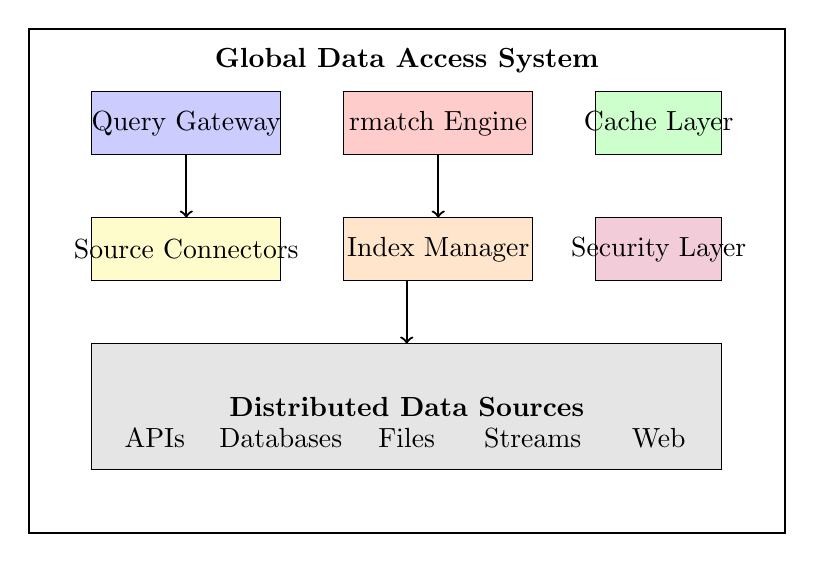
\begin{tikzpicture}[scale=0.8]
  % Draw the main components
  \draw[thick] (0,0) rectangle (12,8);
  \node at (6,7.5) {\textbf{Global Data Access System}};
  
  % Query Gateway
  \draw[fill=blue!20] (1,6) rectangle (4,7);
  \node at (2.5,6.5) {Query Gateway};
  
  % Pattern Matching Engine (rmatch)
  \draw[fill=red!20] (5,6) rectangle (8,7);
  \node at (6.5,6.5) {rmatch Engine};
  
  % Cache Layer
  \draw[fill=green!20] (9,6) rectangle (11,7);
  \node at (10,6.5) {Cache Layer};
  
  % Data Source Connectors
  \draw[fill=yellow!20] (1,4) rectangle (4,5);
  \node at (2.5,4.5) {Source Connectors};
  
  % Index Manager
  \draw[fill=orange!20] (5,4) rectangle (8,5);
  \node at (6.5,4.5) {Index Manager};
  
  % Security Layer
  \draw[fill=purple!20] (9,4) rectangle (11,5);
  \node at (10,4.5) {Security Layer};
  
  % Data Sources
  \draw[fill=gray!20] (1,1) rectangle (11,3);
  \node at (6,2) {\textbf{Distributed Data Sources}};
  \node at (2,1.5) {APIs};
  \node at (4,1.5) {Databases};
  \node at (6,1.5) {Files};
  \node at (8,1.5) {Streams};
  \node at (10,1.5) {Web};
  
  % Arrows
  \draw[->,thick] (2.5,6) -- (2.5,5);
  \draw[->,thick] (6.5,6) -- (6.5,5);
  \draw[->,thick] (6,4) -- (6,3);
\end{tikzpicture}
\caption{GDAS High-Level Architecture}
\end{figure}

\subsubsection{Query Gateway}
Responsible for:
\begin{itemize}
\item Request authentication and authorization
\item Query parsing and optimization
\item Load balancing across processing nodes
\item Response aggregation and formatting
\end{itemize}

\subsubsection{rmatch Pattern Matching Engine}
Core processing component featuring:
\begin{itemize}
\item Combined NFA/DFA automata construction
\item Multi-pattern simultaneous matching
\item Memory-efficient state management
\item Parallel processing capabilities
\end{itemize}

\subsubsection{Data Source Connectors}
Abstraction layer providing:
\begin{itemize}
\item Unified data source interfaces
\item Protocol translation and adaptation
\item Connection pooling and management
\item Error handling and retry logic
\end{itemize}

\subsection{Data Flow Architecture}

The system processes queries through the following stages:

\begin{algorithm}
\caption{Query Processing Pipeline}
\begin{algorithmic}[1]
\Procedure{ProcessQuery}{$query, user\_context$}
    \State $authenticated\_user \gets \Call{Authenticate}{user\_context}$
    \State $parsed\_query \gets \Call{ParseQuery}{query}$
    \State $optimized\_query \gets \Call{OptimizeQuery}{parsed\_query}$
    \State $patterns \gets \Call{ExtractPatterns}{optimized\_query}$
    \State $compiled\_patterns \gets \Call{CompilePatterns}{patterns}$ \Comment{Using rmatch}
    \State $data\_sources \gets \Call{IdentifyDataSources}{optimized\_query}$
    \State $results \gets \Call{ExecuteDistributedQuery}{compiled\_patterns, data\_sources}$
    \State $filtered\_results \gets \Call{ApplySecurityFilters}{results, authenticated\_user}$
    \State $formatted\_response \gets \Call{FormatResponse}{filtered\_results}$
    \State \Return $formatted\_response$
\EndProcedure
\end{algorithmic}
\end{algorithm}

\section{Performance Considerations}

\subsection{rmatch Integration Benefits}

The integration of rmatch provides several performance advantages:

\begin{itemize}
\item \textbf{Deterministic Performance}: No backtracking-related performance cliffs
\item \textbf{Memory Efficiency}: Compact automata representation reduces memory footprint
\item \textbf{Parallel Processing}: Thread-safe pattern matching enables horizontal scaling
\item \textbf{Multi-Pattern Optimization}: Single-pass processing of multiple patterns simultaneously
\end{itemize}

\subsection{Performance Optimization Strategies}

\subsubsection{Pattern Compilation Optimization}
\begin{lstlisting}[language=Java, caption=Optimized Pattern Compilation]
public class OptimizedPatternCompiler {
    private final PatternCache cache;
    private final ExecutorService compilerThreads;
    
    public CompiledPatternSet compile(List<String> patterns) {
        // Check cache first
        String cacheKey = computeCacheKey(patterns);
        CompiledPatternSet cached = cache.get(cacheKey);
        if (cached != null) return cached;
        
        // Parallel compilation for large pattern sets
        if (patterns.size() > PARALLEL_THRESHOLD) {
            return compileInParallel(patterns);
        }
        
        // Single-threaded for small sets
        return compileSingleThreaded(patterns);
    }
}
\end{lstlisting}

\subsubsection{Memory Management}
\begin{itemize}
\item Off-heap caching using Chronicle Map
\item Memory-mapped files for large datasets
\item Generational garbage collection tuning
\item Direct buffer utilization for network I/O
\end{itemize}

\section{Security and Privacy Framework}

\subsection{Data Sovereignty Compliance}
The system implements configurable data sovereignty rules ensuring data remains within specified geographical boundaries while enabling global access patterns.

\subsection{Privacy-Preserving Techniques}
\begin{enumerate}
\item \textbf{Differential Privacy}: Adding controlled noise to query results
\item \textbf{Homomorphic Encryption}: Computing on encrypted data without decryption
\item \textbf{Secure Multi-Party Computation}: Collaborative computation without data sharing
\item \textbf{Zero-Knowledge Proofs}: Proving query results without revealing underlying data
\end{enumerate}

\section{Implementation Roadmap}

\subsection{Phase 1: Foundation (Months 1-6)}
\begin{itemize}
\item Core rmatch integration and optimization
\item Basic data source connector framework
\item Query gateway MVP implementation
\item Security framework foundation
\end{itemize}

\subsection{Phase 2: Scale (Months 7-12)}
\begin{itemize}
\item Distributed caching implementation
\item Advanced indexing strategies
\item Multi-region deployment
\item Performance optimization and tuning
\end{itemize}

\subsection{Phase 3: Intelligence (Months 13-18)}
\begin{itemize}
\item Machine learning-powered query optimization
\item Predictive caching algorithms
\item Advanced analytics and monitoring
\item AI-driven system self-optimization
\end{itemize}

\section{Risk Analysis}

\subsection{Technical Risks}
\begin{longtable}{|p{3cm}|p{3cm}|p{3cm}|p{3cm}|}
\toprule
\textbf{Risk} & \textbf{Impact} & \textbf{Probability} & \textbf{Mitigation} \\
\midrule
State explosion in pattern matching & High & Medium & Use sparse automata representations, pattern simplification \\
\midrule
Network latency variability & Medium & High & Edge caching, request coalescing, adaptive timeouts \\
\midrule
Data source availability & High & Medium & Circuit breakers, graceful degradation, redundant sources \\
\midrule
Regulatory compliance complexity & High & High & Legal review, compliance automation, regular audits \\
\bottomrule
\end{longtable}

\subsection{Business Risks}
\begin{itemize}
\item Market competition from established players
\item Changing regulatory landscape
\item Data source access restrictions
\item Scalability cost challenges
\end{itemize}

\section{Success Metrics and KPIs}

\subsection{Performance Metrics}
\begin{itemize}
\item \textbf{Query Latency}: P95 response time $< 100ms$
\item \textbf{Throughput}: Queries processed per second per node
\item \textbf{Resource Efficiency}: Memory and CPU utilization rates
\item \textbf{Pattern Matching Speed}: Patterns processed per second
\end{itemize}

\subsection{Business Metrics}
\begin{itemize}
\item \textbf{User Adoption}: Monthly active users growth rate
\item \textbf{Data Coverage}: Percentage of available data sources integrated
\item \textbf{Customer Satisfaction}: Net Promoter Score (NPS)
\item \textbf{Revenue Growth}: Annual recurring revenue increase
\end{itemize}

\section{Conclusion}

The Global Data Access System represents a significant advancement in distributed data processing, leveraging rmatch's superior pattern matching capabilities to provide unprecedented performance and scale. The proposed architecture addresses current market limitations while establishing a foundation for future innovation in global data access patterns.

Success depends on careful implementation of the performance-critical components, particularly the rmatch integration, and maintaining focus on the core principles of efficiency, security, and scalability throughout the development process.

\newpage
\appendix

\section{Implementation Hints and Technical Details}

This appendix provides detailed technical guidance for implementing the Global Data Access System, drawing from best practices in high-performance distributed systems and pattern matching optimization.

\subsection{rmatch Integration Patterns}

\subsubsection{Pattern Compilation Optimization}

The core performance advantage of rmatch lies in its automata-based approach. For GDAS, we recommend the following integration patterns:

\begin{lstlisting}[language=Java, caption=Efficient Pattern Set Compilation]
public class GDASPatternCompiler {
    private static final int MAX_PATTERNS_PER_AUTOMATON = 10000;
    private static final int COMPILATION_THREAD_POOL_SIZE = 
        Runtime.getRuntime().availableProcessors() * 2;
    
    private final ExecutorService compilationExecutor;
    private final LoadingCache<PatternSetKey, CompiledAutomaton> cache;
    
    public CompletableFuture<CompiledAutomaton> compilePatterns(
            List<Pattern> patterns) {
        
        // Partition patterns to prevent state explosion
        List<List<Pattern>> partitions = partitionPatterns(patterns);
        
        // Compile partitions in parallel
        List<CompletableFuture<CompiledAutomaton>> futures = 
            partitions.stream()
                .map(partition -> CompletableFuture.supplyAsync(
                    () -> compilePartition(partition), 
                    compilationExecutor))
                .collect(toList());
        
        // Combine results efficiently
        return CompletableFuture.allOf(futures.toArray(new CompletableFuture[0]))
            .thenApply(v -> combineAutomata(
                futures.stream()
                    .map(CompletableFuture::join)
                    .collect(toList())));
    }
    
    private CompiledAutomaton compilePartition(List<Pattern> patterns) {
        // Use rmatch compiler with optimizations
        return RmatchCompiler.newBuilder()
            .withPatterns(patterns)
            .enableStaticOptimizations()
            .enableUnicodeSupport()
            .setMaxStates(100000) // Prevent memory explosion
            .build()
            .compile();
    }
}
\end{lstlisting}

\subsubsection{Memory-Efficient State Management}

GDAS must handle massive pattern sets while maintaining memory efficiency:

\begin{lstlisting}[language=Java, caption=Off-Heap State Storage]
public class OffHeapStateManager {
    private final ChronicleMap<Long, ByteBuffer> stateMap;
    private final DirectByteBufferPool bufferPool;
    
    public OffHeapStateManager(long maxStates, int avgStateSize) {
        this.stateMap = ChronicleMap
            .of(Long.class, ByteBuffer.class)
            .entries(maxStates)
            .averageValueSize(avgStateSize)
            .create();
        this.bufferPool = new DirectByteBufferPool(maxStates, avgStateSize);
    }
    
    public void storeState(long stateId, AutomatonState state) {
        ByteBuffer buffer = bufferPool.acquire();
        try {
            state.serializeTo(buffer);
            buffer.flip();
            stateMap.put(stateId, buffer);
        } finally {
            // Buffer is now owned by ChronicleMap
        }
    }
    
    public AutomatonState loadState(long stateId) {
        ByteBuffer buffer = stateMap.get(stateId);
        return buffer != null ? AutomatonState.deserializeFrom(buffer) : null;
    }
}
\end{lstlisting}

\subsection{Distributed Query Processing}

\subsubsection{Query Sharding Strategy}

Implement intelligent query sharding based on data locality and pattern characteristics:

\begin{lstlisting}[language=Java, caption=Adaptive Query Sharding]
public class AdaptiveQuerySharding {
    
    public List<QueryShard> shardQuery(Query query, List<DataSource> sources) {
        List<QueryShard> shards = new ArrayList<>();
        
        // Analyze patterns for sharding hints
        PatternAnalysis analysis = analyzePatterns(query.getPatterns());
        
        if (analysis.hasLocationConstraints()) {
            // Geographic sharding
            shards.addAll(createGeographicShards(query, sources, analysis));
        } else if (analysis.hasTemporalConstraints()) {
            // Temporal sharding
            shards.addAll(createTemporalShards(query, sources, analysis));
        } else {
            // Content-based sharding
            shards.addAll(createContentBasedShards(query, sources, analysis));
        }
        
        return optimizeShardDistribution(shards);
    }
    
    private List<QueryShard> createContentBasedShards(
            Query query, List<DataSource> sources, PatternAnalysis analysis) {
        
        // Use Bloom filters to eliminate unlikely data sources
        BloomFilter<String> queryTerms = createQueryBloomFilter(query);
        
        return sources.stream()
            .filter(source -> source.getBloomFilter().intersects(queryTerms))
            .map(source -> new QueryShard(query, source, 
                estimateSelectivity(query, source)))
            .sorted(comparing(QueryShard::getSelectivity).reversed())
            .collect(toList());
    }
}
\end{lstlisting}

\subsubsection{Result Aggregation and Deduplication}

Efficiently combine results from distributed shards:

\begin{lstlisting}[language=Java, caption=Streaming Result Aggregation]
public class StreamingResultAggregator {
    private final PriorityQueue<ShardResult> resultQueue;
    private final BloomFilter<String> deduplicationFilter;
    
    public Stream<QueryResult> aggregateResults(
            Stream<CompletableFuture<ShardResult>> shardFutures) {
        
        return shardFutures
            .map(this::awaitResult)
            .filter(Objects::nonNull)
            .flatMap(shardResult -> shardResult.getResults().stream())
            .filter(this::isNotDuplicate)
            .sorted(comparing(QueryResult::getRelevanceScore).reversed())
            .limit(MAX_RESULTS_PER_QUERY);
    }
    
    private boolean isNotDuplicate(QueryResult result) {
        String signature = computeResultSignature(result);
        if (deduplicationFilter.mightContain(signature)) {
            // Potential duplicate, check more expensive exact match
            return !exactDuplicateCheck(result);
        }
        deduplicationFilter.put(signature);
        return true;
    }
}
\end{lstlisting}

\subsection{Performance Optimization Techniques}

\subsubsection{JIT Compilation Optimization}

Optimize for JVM JIT compiler performance:

\begin{lstlisting}[language=Java, caption=JIT-Friendly Pattern Matching]
public class OptimizedMatcher {
    // Use method specialization for common patterns
    private static final int SPECIALIZED_PATTERN_THRESHOLD = 10;
    
    public MatchResult match(CharSequence input, CompiledPattern pattern) {
        // Encourage JIT inlining for hot patterns
        if (pattern.getUsageCount() > SPECIALIZED_PATTERN_THRESHOLD) {
            return matchHotPattern(input, pattern);
        }
        return matchColdPattern(input, pattern);
    }
    
    // Separate methods to enable different JIT optimizations
    private MatchResult matchHotPattern(CharSequence input, CompiledPattern pattern) {
        // Branch-predictable code for frequently used patterns
        return pattern.matchOptimized(input);
    }
    
    private MatchResult matchColdPattern(CharSequence input, CompiledPattern pattern) {
        // Generic implementation for rarely used patterns
        return pattern.match(input);
    }
}
\end{lstlisting}

\subsubsection{CPU Cache Optimization}

Optimize data structures for CPU cache efficiency:

\begin{lstlisting}[language=Java, caption=Cache-Friendly Data Structures]
public class CacheOptimizedAutomaton {
    // Pack state transitions in cache-friendly arrays
    private final int[] transitionTable; // state * alphabet_size + symbol = next_state
    private final boolean[] acceptingStates;
    private final byte[] stateMetadata; // Additional per-state information
    
    public int transition(int currentState, char symbol) {
        // Single array access, cache-friendly
        return transitionTable[currentState * ALPHABET_SIZE + symbol];
    }
    
    public boolean isAccepting(int state) {
        // Direct array access, no indirection
        return acceptingStates[state];
    }
}
\end{lstlisting}

\subsection{Scalability Patterns}

\subsubsection{Reactive Streams Integration}

Use reactive programming for handling massive data streams:

\begin{lstlisting}[language=Java, caption=Reactive Query Processing]
public class ReactiveQueryProcessor {
    
    public Flux<QueryResult> processQuery(Query query) {
        return Flux.fromIterable(query.getDataSources())
            // Parallel processing with backpressure
            .flatMap(source -> processDataSource(source, query)
                .subscribeOn(Schedulers.boundedElastic()), 
                CONCURRENCY_LEVEL)
            // Apply pattern matching
            .transform(this::applyPatternMatching)
            // Handle backpressure
            .onBackpressureBuffer(BUFFER_SIZE, BufferOverflowStrategy.DROP_OLDEST)
            // Aggregate and deduplicate
            .transform(this::aggregateResults);
    }
    
    private Flux<RawData> processDataSource(DataSource source, Query query) {
        return source.createStream(query.getTimeRange())
            .doOnError(error -> handleDataSourceError(source, error))
            .retry(3) // Automatic retry for transient failures
            .timeout(Duration.ofSeconds(30)); // Prevent hanging
    }
}
\end{lstlisting}

\subsection{Monitoring and Observability}

\subsubsection{Performance Metrics Collection}

Implement comprehensive performance monitoring:

\begin{lstlisting}[language=Java, caption=Performance Monitoring]
@Component
public class QueryPerformanceMonitor {
    private final MeterRegistry meterRegistry;
    private final Timer queryTimer;
    private final Counter patternMatches;
    private final Gauge memoryUsage;
    
    public void recordQueryExecution(Query query, Duration executionTime, 
                                   long matchCount, long memoryUsed) {
        // Record timing metrics
        queryTimer.record(executionTime);
        
        // Record match metrics with tags
        patternMatches.increment(Tags.of(
            "query_type", query.getType(),
            "pattern_count", String.valueOf(query.getPatternCount())
        ), matchCount);
        
        // Record memory usage
        memoryUsage.set(memoryUsed);
        
        // Custom metrics for pattern complexity
        recordPatternComplexityMetrics(query);
    }
    
    private void recordPatternComplexityMetrics(Query query) {
        double avgComplexity = query.getPatterns().stream()
            .mapToDouble(this::calculatePatternComplexity)
            .average()
            .orElse(0.0);
            
        Gauge.builder("pattern.complexity.average")
            .tag("query_id", query.getId())
            .register(meterRegistry)
            .set(avgComplexity);
    }
}
\end{lstlisting}

\subsection{Security Implementation Details}

\subsubsection{Query Sanitization}

Implement robust query sanitization to prevent injection attacks:

\begin{lstlisting}[language=Java, caption=Query Security Validation]
public class QuerySecurityValidator {
    private static final int MAX_PATTERN_COMPLEXITY = 10000;
    private static final int MAX_PATTERNS_PER_QUERY = 1000;
    private static final Pattern DANGEROUS_PATTERN = 
        Pattern.compile(".*\\(\\?.*\\(\\?.*"); // Nested lookaheads
    
    public ValidationResult validateQuery(Query query, User user) {
        List<String> violations = new ArrayList<>();
        
        // Check pattern count limits
        if (query.getPatternCount() > MAX_PATTERNS_PER_QUERY) {
            violations.add("Too many patterns in query");
        }
        
        // Check pattern complexity
        for (String pattern : query.getPatterns()) {
            if (calculateComplexity(pattern) > MAX_PATTERN_COMPLEXITY) {
                violations.add("Pattern too complex: " + pattern);
            }
            
            if (DANGEROUS_PATTERN.matcher(pattern).matches()) {
                violations.add("Potentially dangerous pattern: " + pattern);
            }
        }
        
        // Check user permissions
        if (!hasPermission(user, query.getDataSources())) {
            violations.add("Insufficient permissions");
        }
        
        return violations.isEmpty() ? 
            ValidationResult.valid() : 
            ValidationResult.invalid(violations);
    }
}
\end{lstlisting}

\subsubsection{Data Encryption and Privacy}

Implement end-to-end encryption for sensitive data:

\begin{lstlisting}[language=Java, caption=Privacy-Preserving Data Processing]
public class PrivacyAwareDataProcessor {
    private final EncryptionService encryptionService;
    private final DifferentialPrivacyEngine privacyEngine;
    
    public ProcessedData processWithPrivacy(RawData data, PrivacyLevel level) {
        switch (level) {
            case PUBLIC:
                return processPlaintext(data);
                
            case CONFIDENTIAL:
                // Process encrypted data using homomorphic encryption
                return processEncrypted(data);
                
            case HIGHLY_SENSITIVE:
                // Use secure multi-party computation
                return processWithSMPC(data);
                
            default:
                throw new IllegalArgumentException("Unsupported privacy level");
        }
    }
    
    private ProcessedData processEncrypted(RawData data) {
        // Homomorphic encryption allows computation on encrypted data
        EncryptedData encryptedData = encryptionService.encrypt(data);
        EncryptedResult result = performHomomorphicComputation(encryptedData);
        
        // Add differential privacy noise
        return privacyEngine.addNoise(result, PRIVACY_BUDGET);
    }
}
\end{lstlisting}

\subsection{Data Source Integration Patterns}

\subsubsection{Adaptive Protocol Handling}

Implement flexible protocol adapters for different data sources:

\begin{lstlisting}[language=Java, caption=Universal Data Source Adapter]
public abstract class DataSourceAdapter<T> {
    protected final ConnectionPool connectionPool;
    protected final CircuitBreaker circuitBreaker;
    protected final RateLimiter rateLimiter;
    
    public abstract CompletableFuture<Stream<T>> query(
        AdapterQuery query, QueryContext context);
    
    protected <R> CompletableFuture<R> executeWithResilience(
            Supplier<CompletableFuture<R>> operation) {
        
        return circuitBreaker.executeSupplier(() ->
            rateLimiter.executeSupplier(operation))
            .exceptionally(throwable -> {
                logError(throwable);
                return getDefaultValue();
            });
    }
}

@Component
public class DatabaseAdapter extends DataSourceAdapter<DatabaseRecord> {
    
    @Override
    public CompletableFuture<Stream<DatabaseRecord>> query(
            AdapterQuery query, QueryContext context) {
        
        return executeWithResilience(() ->
            CompletableFuture.supplyAsync(() -> {
                String sql = translateToSQL(query);
                return executeSQL(sql).stream();
            }));
    }
    
    private String translateToSQL(AdapterQuery query) {
        // Convert universal query to SQL
        SQLQueryBuilder builder = new SQLQueryBuilder();
        return builder
            .select(query.getProjection())
            .from(query.getTables())
            .where(translatePatterns(query.getPatterns()))
            .limit(query.getLimit())
            .build();
    }
}
\end{lstlisting}

\subsection{Advanced Caching Strategies}

\subsubsection{Intelligent Cache Warming}

Implement predictive cache warming based on query patterns:

\begin{lstlisting}[language=Java, caption=Predictive Cache Warming]
public class PredictiveCacheWarmer {
    private final MachineLearningPredictor predictor;
    private final CacheService cacheService;
    private final ScheduledExecutorService scheduler;
    
    @PostConstruct
    public void initializeCacheWarming() {
        // Schedule regular cache warming
        scheduler.scheduleWithFixedDelay(
            this::warmFrequentlyAccessedData,
            0, 5, TimeUnit.MINUTES);
    }
    
    public void warmFrequentlyAccessedData() {
        List<QueryPrediction> predictions = 
            predictor.predictNextQueries(Instant.now().plusMinutes(30));
        
        predictions.parallelStream()
            .filter(pred -> pred.getConfidence() > 0.7)
            .forEach(this::preloadQueryData);
    }
    
    private void preloadQueryData(QueryPrediction prediction) {
        Query query = prediction.getQuery();
        String cacheKey = generateCacheKey(query);
        
        if (!cacheService.contains(cacheKey)) {
            // Asynchronously warm cache
            CompletableFuture.runAsync(() -> {
                QueryResult result = executeQuery(query);
                cacheService.put(cacheKey, result, 
                    Duration.ofMinutes(30));
            });
        }
    }
}
\end{lstlisting}

\subsection{Testing and Validation Strategies}

\subsubsection{Performance Testing Framework}

Implement comprehensive performance testing using JMH:

\begin{lstlisting}[language=Java, caption=JMH Performance Testing]
@BenchmarkMode(Mode.Throughput)
@OutputTimeUnit(TimeUnit.SECONDS)
@State(Scope.Benchmark)
@Fork(value = 2, jvmArgs = {"-Xms4G", "-Xmx4G"})
@Warmup(iterations = 3, time = 10, timeUnit = TimeUnit.SECONDS)
@Measurement(iterations = 5, time = 10, timeUnit = TimeUnit.SECONDS)
public class GDASPerformanceBenchmark {
    
    private QueryProcessor queryProcessor;
    private List<Query> testQueries;
    private List<DataSource> mockDataSources;
    
    @Setup
    public void setup() {
        queryProcessor = new QueryProcessor();
        testQueries = generateTestQueries(1000);
        mockDataSources = createMockDataSources(100);
    }
    
    @Benchmark
    public int benchmarkSimplePatternMatching(Blackhole bh) {
        Query query = testQueries.get(ThreadLocalRandom.current()
            .nextInt(testQueries.size()));
        
        QueryResult result = queryProcessor.process(query);
        bh.consume(result);
        return result.getMatchCount();
    }
    
    @Benchmark
    @Group("mixed_workload")
    @GroupThreads(8)
    public void benchmarkMixedQueries(Blackhole bh) {
        // Simulate real-world mixed query patterns
        Query query = selectWeightedRandomQuery();
        QueryResult result = queryProcessor.process(query);
        bh.consume(result);
    }
}
\end{lstlisting}

\subsubsection{Chaos Engineering Integration}

Implement chaos engineering to validate system resilience:

\begin{lstlisting}[language=Java, caption=Chaos Engineering Framework]
@Component
public class ChaosEngineeringController {
    
    @EventListener
    @ConditionalOnProperty("chaos.enabled")
    public void introduceRandomFailures(QueryProcessingEvent event) {
        if (ThreadLocalRandom.current().nextDouble() < FAILURE_RATE) {
            ChaosExperiment experiment = selectRandomExperiment();
            experiment.execute(event.getQuery());
        }
    }
    
    private enum ChaosExperiment {
        NETWORK_LATENCY {
            @Override
            void execute(Query query) {
                // Introduce artificial network delays
                addNetworkLatency(Duration.ofMillis(
                    ThreadLocalRandom.current().nextInt(100, 1000)));
            }
        },
        
        DATA_SOURCE_FAILURE {
            @Override
            void execute(Query query) {
                // Simulate data source unavailability
                DataSource randomSource = selectRandomDataSource(query);
                temporarilyDisableDataSource(randomSource, 
                    Duration.ofMinutes(1));
            }
        },
        
        MEMORY_PRESSURE {
            @Override
            void execute(Query query) {
                // Create memory pressure
                allocateMemory(1024 * 1024 * 100); // 100MB
            }
        };
        
        abstract void execute(Query query);
    }
}
\end{lstlisting}

\bibliographystyle{plainnat}
\bibliography{references}

\end{document}